%\title{LaTeX Portrait Poster Template}
%%%%%%%%%%%%%%%%%%%%%%%%%%%%%%%%%%%%%%%%%
% a0poster Portrait Poster
% LaTeX Template
% Version 1.0 (22/06/13)
%
% The a0poster class was created by:
% Gerlinde Kettl and Matthias Weiser (tex@kettl.de)
% 
% This template has been downloaded from:
% http://www.LaTeXTemplates.com
%
% License:
% CC BY-NC-SA 3.0 (http://creativecommons.org/licenses/by-nc-sa/3.0/)
%
%%%%%%%%%%%%%%%%%%%%%%%%%%%%%%%%%%%%%%%%%

%----------------------------------------------------------------------------------------
%	PACKAGES AND OTHER DOCUMENT CONFIGURATIONS
%----------------------------------------------------------------------------------------

\documentclass[a0,portrait]{a0poster}

\usepackage{multicol} % This is so we can have multiple columns of text side-by-side
\columnsep=100pt % This is the amount of white space between the columns in the poster
\columnseprule=3pt % This is the thickness of the black line between the columns in the poster

\usepackage[svgnames]{xcolor} % Specify colors by their 'svgnames', for a full list of all colors available see here: http://www.latextemplates.com/svgnames-colors

\usepackage{times} % Use the times font
%\usepackage{palatino} % Uncomment to use the Palatino font

\usepackage{graphicx} % Required for including images
\graphicspath{{Assets/}} % Location of the graphics files
\usepackage{booktabs} % Top and bottom rules for table
\usepackage[font=small,labelfont=bf]{caption} % Required for specifying captions to tables and figures
\usepackage{amsfonts, amsmath, amsthm, amssymb} % For math fonts, symbols and environments
\usepackage{wrapfig} % Allows wrapping text around tables and figures


\begin{document}

%----------------------------------------------------------------------------------------
%	POSTER HEADER 
%----------------------------------------------------------------------------------------

% The header is divided into two boxes:
% The first is 75% wide and houses the title, subtitle, names, university/organization and contact information
% The second is 25% wide and houses a logo for your university/organization or a photo of you
% The widths of these boxes can be easily edited to accommodate your content as you see fit

\begin{minipage}[b]{0.72\linewidth}
\Huge \color{NavyBlue} \textbf{Profile Guided Source Coding in Compiler Optimization} \color{Black}\\ % Title
\LARGE \textit{An Approach to Reduce The Run-time Memory Occupancy}\\[2cm] % Subtitle
\LARGE \textbf{Chenhao Wu}\\[0.5cm] % Author(s)
\LARGE The Chinese University of Hong Kong, Shenzhen\\School of Science and Engineering\\[0.4cm] % University/organization
\Large \texttt{chenhaowu@link.cuhk.edu.cn}\\
\end{minipage}
%
\begin{minipage}[b]{0.25\linewidth}

\includegraphics[width=20cm]{cuhksz.png}

\includegraphics[width=20cm]{iotlab}
\end{minipage}

\vspace{1cm} % A bit of extra whitespace between the header and poster content

%----------------------------------------------------------------------------------------

\begin{multicols}{2} % This is how many columns your poster will be broken into, a portrait poster is generally split into 2 columns

%----------------------------------------------------------------------------------------
%	ABSTRACT
%----------------------------------------------------------------------------------------

\color{Navy} % Navy color for the abstract

\begin{abstract}
\normalsize
In order to best utilize the run-time memory occupancy and to give powerful and intensive memory-consumption applications with higher compatibility on mobile and embedded systems, we proposed a compiler optimization, Profile Guided Source Coding (PGSC), which is led by the compilation process and aims to reduce the run-time memory occupancy of compiled programs. The optimization of PGSC is based on a profile generated by sample runs on the initially compiled executable, and the profile entails the access (load/read) frequencies on the allocated memory blocks performed by the program during run-time. Our strategy is during the compilation the memory accessing instructions of the program will be substituted by compress and decompress instructions, such that the memory blocks with lower frequency will be compressed into a compressed area when idled and will be decompressed into a run-time area when they are to be loaded. To achieve this objective we apply the Lempel-Ziv coding on the compression process and artificially selected several sample programs as the benchmark to examine the performance of programs compiled with PGSC optimization. The experiment shows that after applying PGSC optimization the average memory occupancy (AMO) and the maximum memory occupancy (MMO) of the identical program are decreased. Even though it would also bring an additional overhead in distributing the computing resources in run-time compression and decompression, the experiment shows this optimization is considerable in practice. In the future, we will research on the combination of the PGSC optimization and the distributed cache system, and also the investigation on the capability of combining PGSC optimization with contemporary channel coding schemes. 

\end{abstract}

%----------------------------------------------------------------------------------------
%	INTRODUCTION
%----------------------------------------------------------------------------------------

\color{SaddleBrown} % SaddleBrown color for the introduction

\section*{Introduction}

In the past two decades, the computing performance of mobile and embedded systems have been significantly raised such that more computing workloads can be undertaken on mobiles and embedded systems, such as digital image processing, machine learning \& deep learning algorithms, augmented-reality applications, and so on. In practice, one of the critical bottlenecks in mobiles and embedded systems design and optimizations is the run-time memory space and power consumption. Since the complexity of program and data set grew much faster than the amelioration of hardware, rather than using expensive electronic components to fulfill the increasing demand of computation resource, it is more promising to find approaches to best utilize the system use of memory space. To achieve this objective, we proposed a Profile Guided Source Coding (PGSC) optimization that will perform an adaptive data compression on allocated memory space during run-time according to different applications and run-time environment. 

\color{DarkSlateGray} % DarkSlateGray color for the rest of the content

\section*{Profile Guided Compilation}
\vspace{1cm}

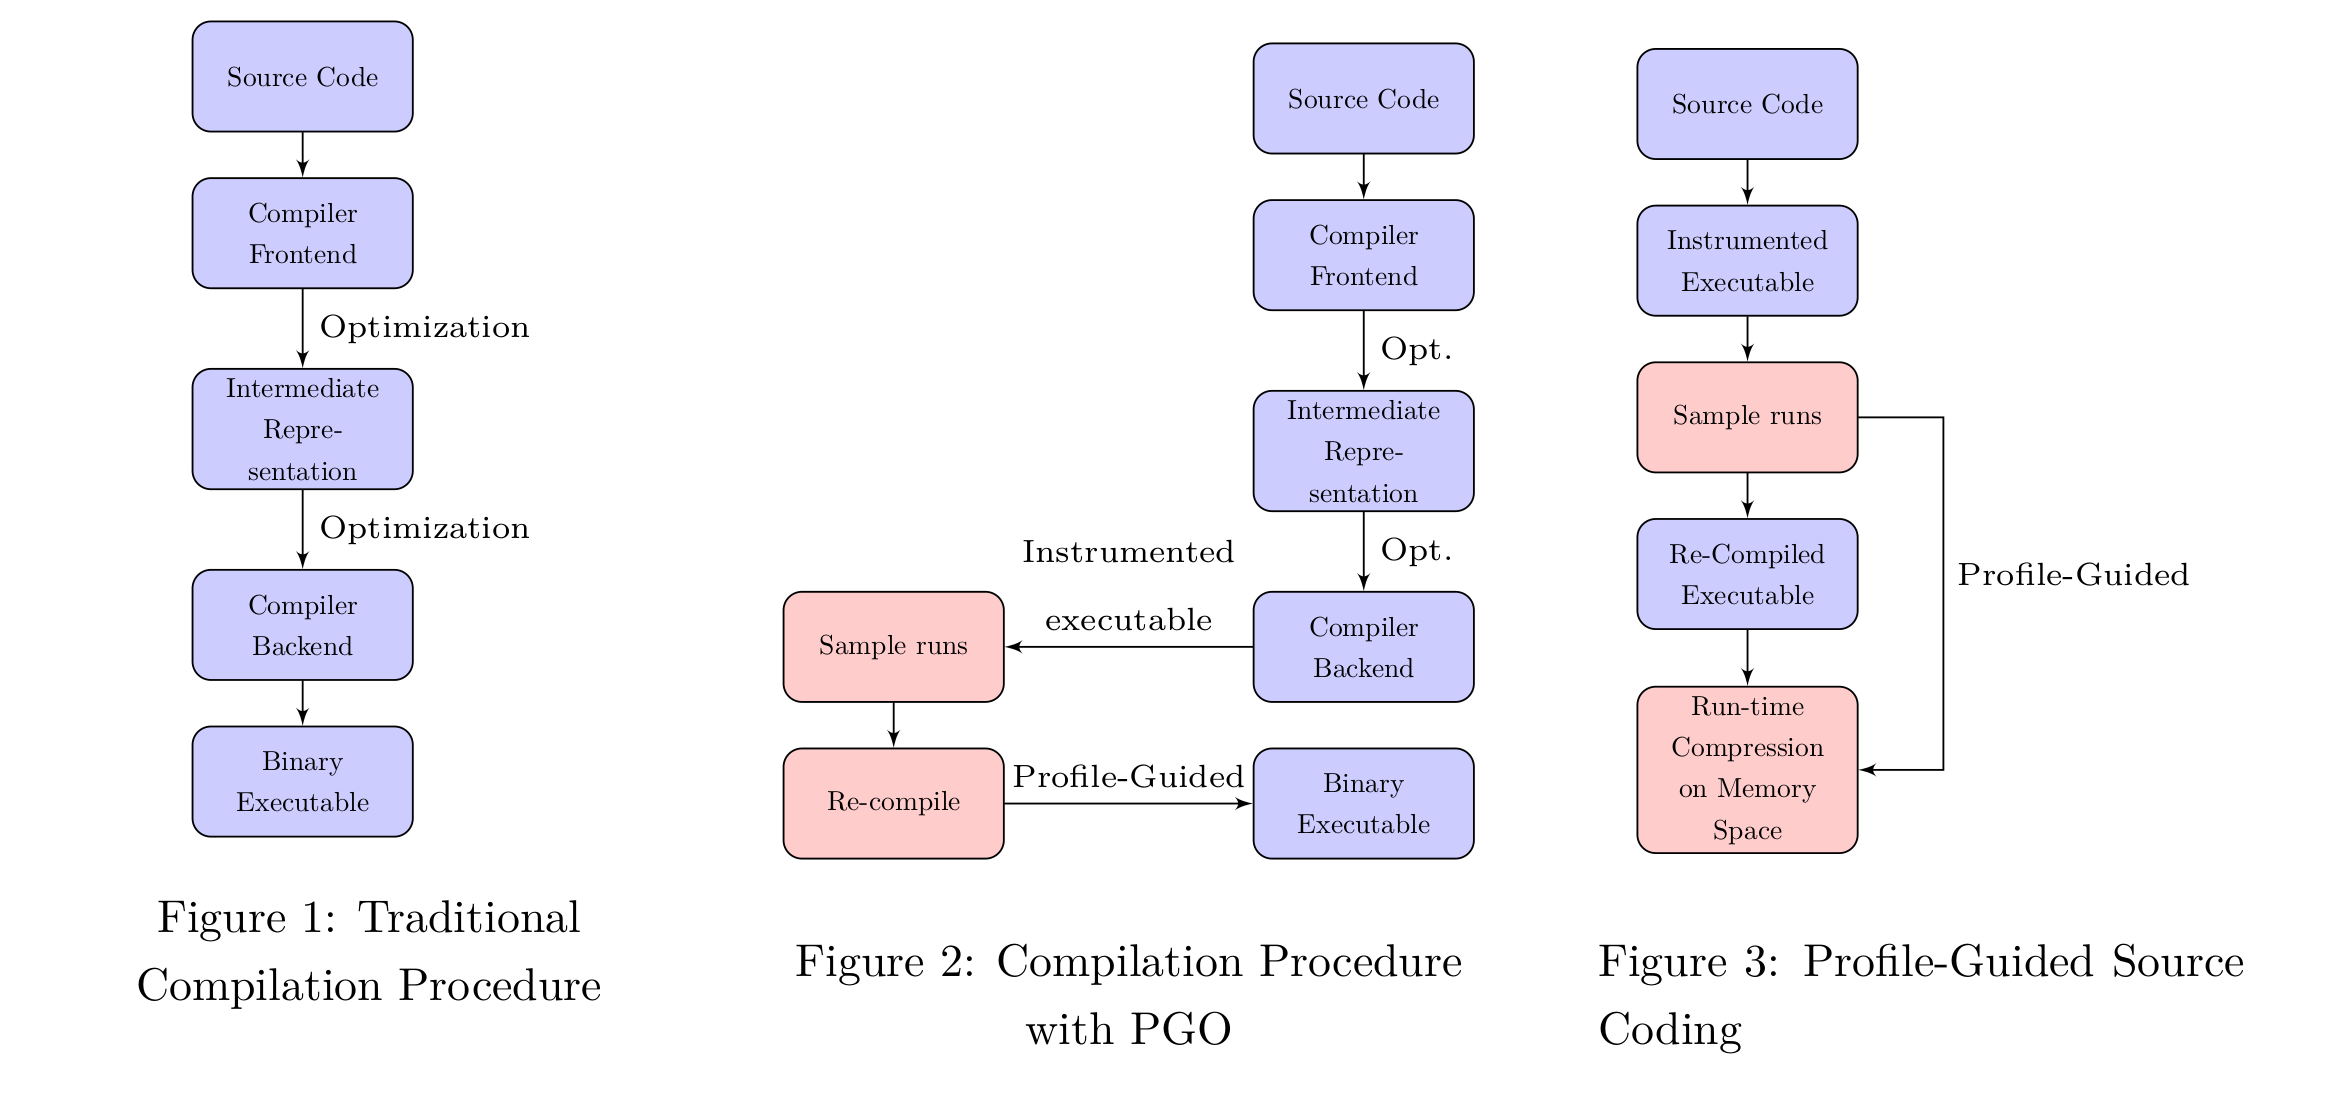
\includegraphics[width=\linewidth]{fig1}

\vspace{1cm}

Inspired by Profile Guided Optimization, the optimization of PGSC requires profiling the compiled executable so as to amend the programs adapting to the run-time behaviors. As shown in Figure 1 and Figure 2, differed from the traditional compilation process, the compiler with profile guided optimization performs a recompilation based on a profile generated by sample runs on initial executable, and applies optimizations according to the profile. 

\section*{Workflow of PGSC}

\begin{enumerate}
	\item Apply the generic compiler to guide the initial compilation and transform the source code into binary executable
	\item Analyze sample runs of the program, profiling the heap access frequency
	\item Pass the profile to compiler and rewrite instruction according to the profile
\end{enumerate}
%----------------------------------------------------------------------------------------
%	MATERIALS AND METHODS
%----------------------------------------------------------------------------------------

\section*{Run-time Compression \& Decompression}

In the PGSC scheme during run-time the memory space will be separated into two areas, run-time area and compressed area.
\vspace{1cm}

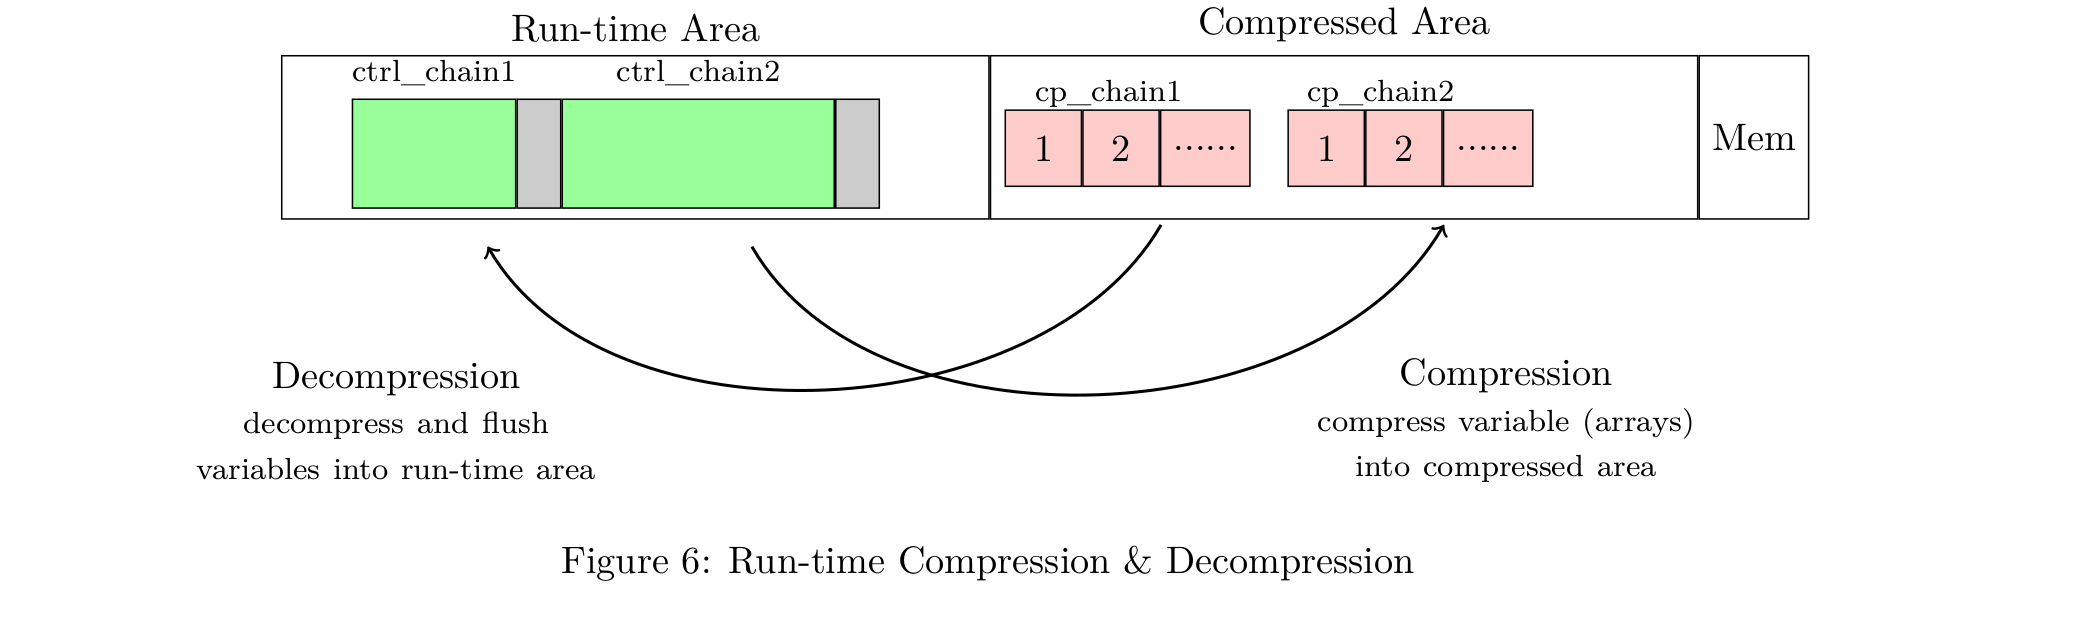
\includegraphics[width=\linewidth]{fig2}

\vspace{1cm}

In the compilation, the compiler specifies the areas of data to be compressed during idle time, and also generates codeword for each block so as during run-time the program would automatically compress them from the run-time area into the compressed area. Whenever the compressed data are to be loaded, the program will instantaneously decompress the data from the compressed area, and flush into the run-time area.  

%----------------------------------------------------------------------------------------
%	RESULTS 
%----------------------------------------------------------------------------------------

\section*{Experiments \& Results}

To examine the performance of programs compiled with PGSC optimization, we apply several testing programs to present a comparison between programs compiled with PGSC and programs without PGSC.

\vspace{1cm}
\textbf{Testing Environment}

\begin{itemize}
	\item \textbf{Operating System}: Debian 9 x86-64 virtual machine 
	\item \textbf{RAM}: 512 MB
	\item \textbf{Number of Processors}: 1
	\item \textbf{Clock Frequency}: 2.8 GHz
	\item \textbf{Generic Compiler}: clang/clang++
\end{itemize}

\vspace{1cm}

\textbf{Results}
\begin{center}
	\begin{tabular}{l l l l l l l}
		\toprule
		\textbf{Program} & \textbf{Functionality} &
		\begin{tabular}{@{}c@{}} \textbf{MMO} \\ \textbf{(clang)} \end{tabular} & 
		\begin{tabular}{@{}c@{}} \textbf{AMO} \\ \textbf{(clang)} \end{tabular} & 
		\begin{tabular}{@{}c@{}} \textbf{MMO} \\ \textbf{(PGSC)} \end{tabular} & 
		\begin{tabular}{@{}c@{}} \textbf{AMO} \\ \textbf{(PGSC)} \end{tabular} & 
		\begin{tabular}{@{}c@{}} \textbf{Extra} \\ \textbf{Terminating Time} \end{tabular} \\
		\midrule\\
		LU-Dec & \begin{tabular}{@{}c@{}}\small Solve a set of linear eqs.\\ \small using LU decomposition\end{tabular} & 214.3 Mb & 165.7 Mb & 153.7 Mb & 53.9 Mb & \hspace{2cm} +47\% \\\\
		Face-Rec & \begin{tabular}{@{}c@{}}\small Learn new faces captured \\ \small from webcam\end{tabular} & 470.0 Mb & 365.2 Mb & 217.8 Mb & 93.7 Mb & \hspace{1.8cm} +239\% \\\\
		LZO & \begin{tabular}{@{}c@{}}\small Compress sample text files \\ \small using LZO algorithms\end{tabular} & 253.7 Mb & 103.8 Mb & 217.8 Mb & 93.7 Mb & \hspace{2cm} +65\% \\\\
		Huff-Cod & \begin{tabular}{@{}c@{}}\small Compress sample text files\\ \small using Huffman Coding\end{tabular} & 324.1 Mb & 214.7 Mb & 293.7 Mb & 196.5 Mb & \hspace{2cm} +53\%
		\\\\
		\bottomrule
	\end{tabular}
\end{center}

\vspace{1cm}

From the result of experiments, both the maximum memory occupancy and the average memory occupancy are shown to decrease after applying PGSC optimization. For the LU Decomposition program and the Facial Recognition program the decrease rate is more remarkable than the rest two testing programs. Due to the basic algorithms the former two programs tend to store lots of intermediate matrices or intermediate picture data on the heap. Thus, the experiment result also implies the run-time compression can achieve better optimization for programs that store more intermediate and redundant data on the heap. 
\\\\
Even though the extra compression time and terminating time have been increased after applied PGSC in the compilation, the overhead is still within an acceptable range. Hence, applying run-time compression as a optimization is considerable for programs.

%----------------------------------------------------------------------------------------
%	FORTHCOMING RESEARCH
%----------------------------------------------------------------------------------------

\section*{Forthcoming Research}
The current process of PGSC we proposed are still being performed on a single computer, as well as all the experiments involved. However, it is still feasible to apply such a compiler-directed technique to a distributed system, because during run-time the memory space has been virtually divided into two partitions after PGSC optimization. Hence, our future research will focus on applying this technique to distributed systems, and also to investigate the capability of combining PGSC optimization with contemporary channel coding schemes. In addition, we will also take efforts to enhance the computational efficiency of PGSC in order to decrease the additional overhead. 

 %----------------------------------------------------------------------------------------
%	REFERENCES
%----------------------------------------------------------------------------------------

\nocite{*} % Print all references regardless of whether they were cited in the poster or not
\bibliographystyle{plain} % Plain referencing style
\bibliography{sample} % Use the example bibliography file sample.bib

%----------------------------------------------------------------------------------------
%	ACKNOWLEDGEMENTS
%----------------------------------------------------------------------------------------

%\section*{Acknowledgments}


%----------------------------------------------------------------------------------------

\end{multicols}
\end{document}